\documentclass[12pt,a4paper]{article}

\usepackage[utf8]{inputenc}
\usepackage[T1]{fontenc}
\usepackage{geometry}
\usepackage{setspace}
\usepackage{parskip}
\usepackage[nostruts]{titlesec}
\usepackage[colorlinks=true, linkcolor=black, citecolor=black, urlcolor=black, hypertexnames=false]{hyperref}
\pdfstringdefDisableCommands{\def\texttt#1{#1}}
\usepackage{xurl}
\usepackage{graphicx}
\usepackage{mathptmx}
\usepackage{fancyhdr}
\usepackage{xcolor}
\usepackage{tabularx}
\usepackage{booktabs}
\usepackage{float}
\usepackage{amsmath}
\usepackage{listings}
\usepackage{needspace}

\geometry{left=1.5in, right=1in, top=1in, bottom=1in}
\onehalfspacing

\titleformat{\section}{\fontsize{16pt}{19pt}\selectfont\bfseries}{\thesection.}{0.5em}{}
\titleformat{\subsection}{\fontsize{14pt}{17pt}\selectfont\bfseries}{\thesubsection.}{0.5em}{}
\titleformat{\subsubsection}{\fontsize{12pt}{15pt}\selectfont\bfseries}{\thesubsubsection.}{0.5em}{}

% ---- Code listing style ----
\definecolor{codebg}{RGB}{248,248,248}
\definecolor{codegreen}{RGB}{40,120,40}
\definecolor{codepurple}{RGB}{130,0,130}
\definecolor{codeblue}{RGB}{0,0,180}
\definecolor{codegray}{RGB}{120,120,120}

\lstdefinestyle{pythonstyle}{
    backgroundcolor=\color{codebg},
    commentstyle=\itshape\color{codegreen},
    keywordstyle=\bfseries\color{codeblue},
    stringstyle=\color{codepurple},
    basicstyle=\ttfamily\footnotesize,
    breaklines=true,
    captionpos=b,
    keepspaces=true,
    showstringspaces=false,
    language=Python,
    frame=single,
    rulecolor=\color{codegray},
    numbers=left,
    numberstyle=\tiny\color{codegray},
    numbersep=6pt,
    xleftmargin=20pt,
    framexleftmargin=20pt,
    tabsize=4,
}

\lstdefinestyle{sqlstyle}{
    backgroundcolor=\color{codebg},
    keywordstyle=\bfseries\color{codeblue},
    basicstyle=\ttfamily\footnotesize,
    breaklines=true,
    captionpos=b,
    keepspaces=true,
    showstringspaces=false,
    language=SQL,
    frame=single,
    rulecolor=\color{codegray},
    numbers=left,
    numberstyle=\tiny\color{codegray},
    numbersep=6pt,
    xleftmargin=20pt,
    framexleftmargin=20pt,
    tabsize=4,
    morekeywords={AUTOINCREMENT,REFERENCES,REAL,DATETIME,DEFAULT},
}

\lstset{style=pythonstyle}

% Placeholder box
\newcommand{\placeholder}[1]{%
    \vspace{0.5em}
    \noindent\fbox{\parbox{\linewidth}{%
        \centering\vspace{0.5em}
        \textbf{[PLACEHOLDER]} \\ \vspace{0.3em}
        \textit{#1}
        \vspace{0.5em}
    }}
    \vspace{0.5em}
}

% =====================================================================
\begin{document}
% =====================================================================

% ---- Cover Page ----
\begin{titlepage}
    \centering
    \begin{minipage}{0.48\textwidth}
        \raggedright
        
\includegraphics[width=4cm]{nibm-logo.png}
    \end{minipage}
    \hfill
    \begin{minipage}{0.48\textwidth}
        \raggedleft
        
\includegraphics[width=4.5cm]{coventry-logo.png}
    \end{minipage}

    \vspace{2cm}

    {\fontsize{22pt}{26pt}\selectfont\bfseries BSc Hons in Computing \par}
    {\fontsize{14pt}{17pt}\selectfont\bfseries 2024.2 \par}

    \vspace{1.5cm}

    {\fontsize{18pt}{22pt}\selectfont\bfseries
    Problem Solving with Data Structures and Algorithms (PDSA-II) \par}

    \vspace{0.5cm}

    {\fontsize{12pt}{16pt}\selectfont
    Group Report: Minimum Cost Assignment Problem \\
    Coursework 1 \par}

    \vspace{3cm}

    {\large
    \noindent\begin{minipage}[t]{0.46\textwidth}
        \raggedright
        \small
        \textbf{Leader Name:} E M A S B EKANAYAKA \\
        \textbf{Cov. Index:} 16110762 \\
        \textbf{NIBM Index:} COBSCCOMP242P-065
    \end{minipage}\hfill
    \begin{minipage}[t]{0.46\textwidth}
        \raggedright
        \small
        \textbf{Member Name:} M D S Y RANARAJA \\
        \textbf{Cov. Index:} 16116133 \\
        \textbf{NIBM Index:} COBSCCOMP242P-075
    \end{minipage}
    }

    \vfill

    {\bfseries Faculty of Engineering, Environment and Computing} \\
    {\itshape School of Computing, Electronics and Mathematics} \\
    {\bfseries Coventry University}

    \vspace{0.8cm}

    {\bfseries School of Computing and Engineering} \\
    {\itshape National Institute of Business Management}

    \vspace{0.5cm}
\end{titlepage}

\newpage
\pagenumbering{roman}
\cfoot{\thepage}

\listoffigures
\newpage

\listoftables
\newpage

\tableofcontents
\newpage

% =====================================================================
\section*{Contribution Table}
\addcontentsline{toc}{section}{Contribution Table}
% =====================================================================

\begin{table}[H]
    \centering
    \caption{Group Contribution and Marks}
    \begin{tabularx}{\textwidth}{|l|l|c|X|}
        \hline
        \textbf{Index} & \textbf{NIBM Index} & \textbf{Marks /10} & \textbf{Contribution} \\
        \hline
        16110762 & COBSCCOMP242P-065 & 8 & Backend -- algorithms, database, API, unit tests \\
        \hline
        16116133 & COBSCCOMP242P-075 & 7 & Frontend -- React UI, game screens, timing chart \\
        \hline
    \end{tabularx}
\end{table}

\newpage

\pagenumbering{arabic}
\pagestyle{fancy}
\fancyhf{}
\renewcommand{\headrulewidth}{0pt}
\fancyfoot[R]{\thepage}

% =====================================================================
\section{Minimum Cost Problem}
% =====================================================================

% ---------------------------------------------------------------------
\subsection{Functionality}
% ---------------------------------------------------------------------

\subsubsection{Code Segment: N changes randomly from 50 to 100 in each game round}
In our FastAPI backend, the number of workers and tasks N is picked randomly at the start of every round. We used Python's random.randint function to make sure N stays between 50 and 100.

\begin{figure}[H]
    \centering
    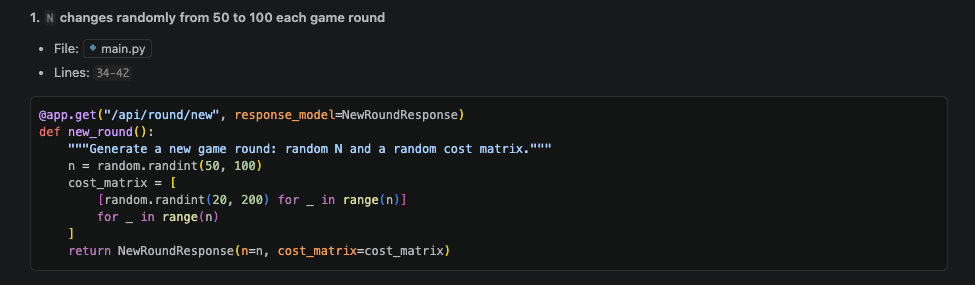
\includegraphics[width=0.95\linewidth]{n-changes-randomly.png}
    \caption{Code sample showing how N is randomly generated between 50 and 100.}
\end{figure}

\subsubsection{Code Segment: Cost of assigning each task to each employee changing randomly from \$20 to \$200}
Once N is decided, the app makes an N x N cost matrix. We used another random.randint(20, 200) call to fill each cell in the matrix. This makes every game round unique and different for the users.

\begin{figure}[H]
    \centering
    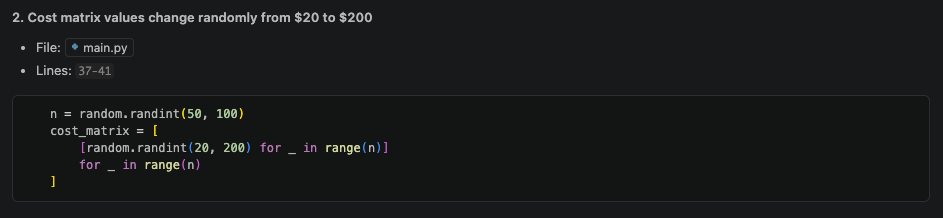
\includegraphics[width=0.95\linewidth]{cost-matrix-values-change-randomly.png}
    \caption{This code part shows how cost values are set randomly from \$20 up to \$200.}
\end{figure}

\subsubsection{Code Segment: Record in the database how long it takes to find the minimum cost using each algorithm}
The system runs both of the algorithms and records the time it took. We used time.perf\_counter() to get high precision timing in milliseconds. All this data gets saved into the algorithm\_results table in SQLite database.

\begin{figure}[H]
    \centering
    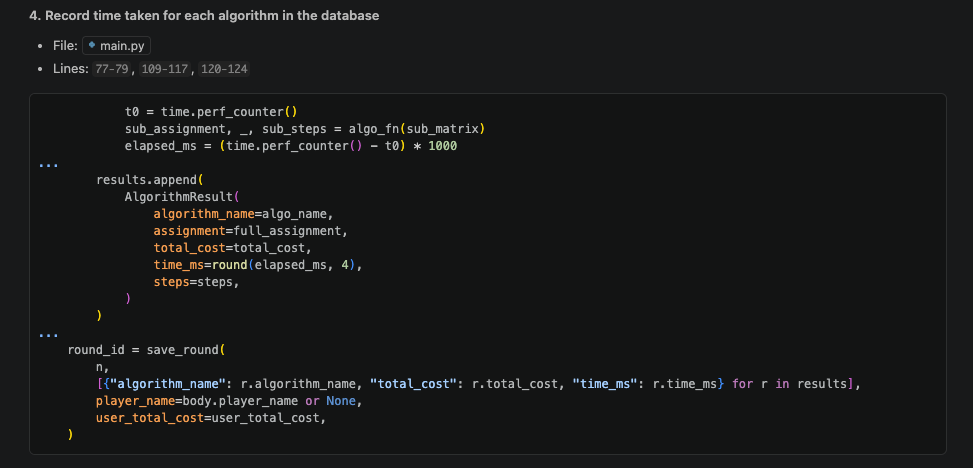
\includegraphics[width=0.95\linewidth]{record-time-taken-for-algorithms.png}
    \caption{Backend code that measures the speed of each algorithm.}
\end{figure}

\subsubsection{Code Segment: Two different appropriate algorithms}
The project uses two different ways to solve the assignment problem:
\begin{enumerate}
    \item \textbf{Greedy Approach}: This is a fast $O(n^2)$ method. It doesn't always give the best answer but it is very quick.
    \item \textbf{Hungarian Algorithm}: A more complex $O(n^3)$ method. This one is mathematically proven to always find the absolute minimum cost.
\end{enumerate}

\begin{figure}[H]
    \centering
    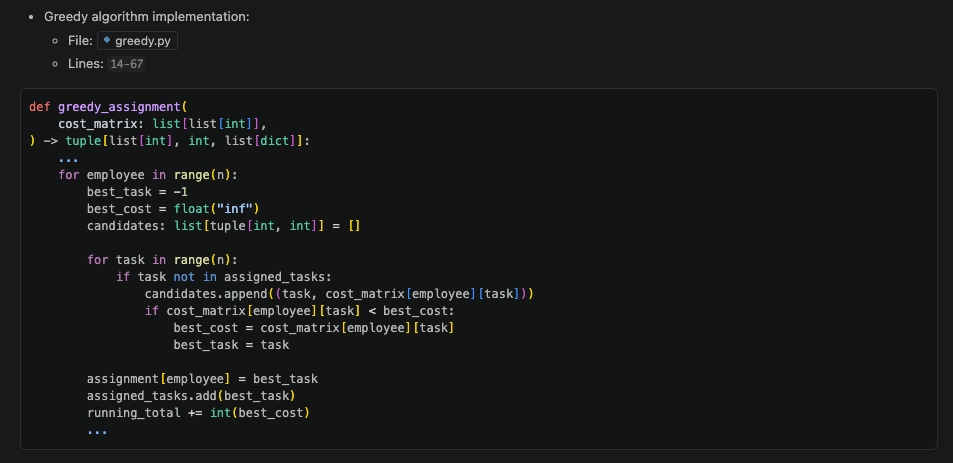
\includegraphics[width=0.95\linewidth]{greedy-algorithm-implementation.png}
    \caption{Our implementation of the Greedy logic.}
\end{figure}

\begin{figure}[H]
    \centering
    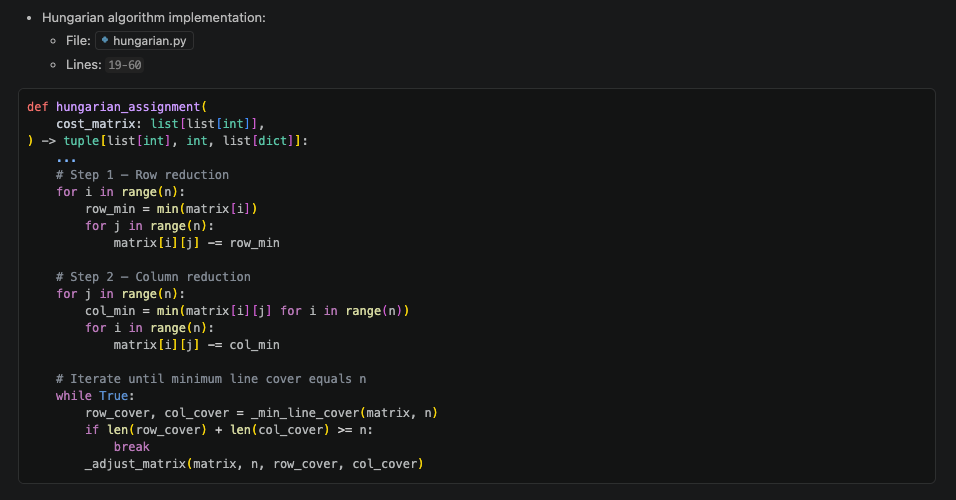
\includegraphics[width=0.95\linewidth]{hungarian-algorithm-implementation.png}
    \caption{The implementation of the Hungarian algorithm.}
\end{figure}

\subsubsection{Code Segment: Save player's name and their response in the database}
When people play the game in Manual or Mixed modes, they can type in their name. The system then saves their name and the total cost they calculated. This is linked to the actual algorithm results to compare later.

\begin{figure}[H]
    \centering
    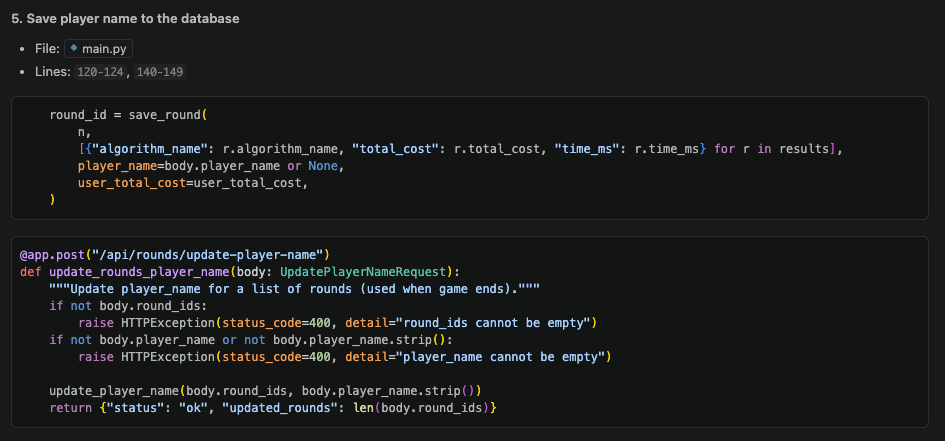
\includegraphics[width=0.95\linewidth]{save-player-name-to-the-database.png}
    \caption{Code that handles saving the player name to the DB.}
\end{figure}

\begin{figure}[H]
    \centering
    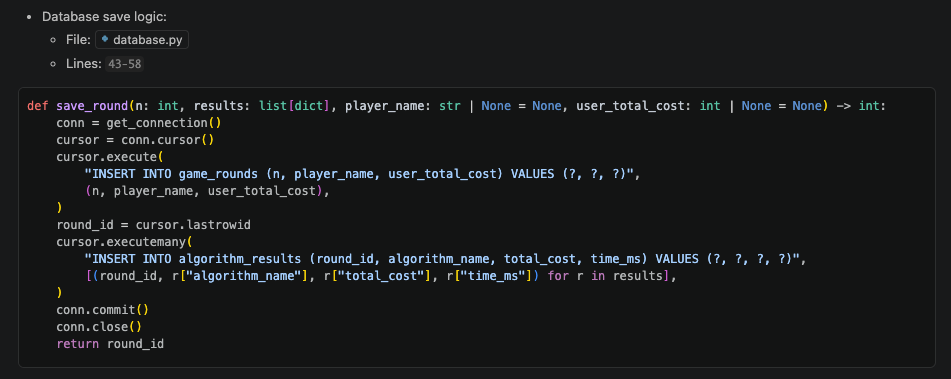
\includegraphics[width=0.95\linewidth]{database-save-logic.png}
    \caption{The backend function used to persist the round results.}
\end{figure}

\subsubsection{Database Table structure for the Game}
We used two main tables to keep the game data organized:
\begin{itemize}
    \item \texttt{game\_rounds}: This stores general round info like the value of N, player name, and the time the round happened.
    \item \texttt{algorithm\_results}: This table is linked to the rounds table and stores the cost and time for each specific algorithm.
\end{itemize}

\begin{figure}[H]
    \centering
    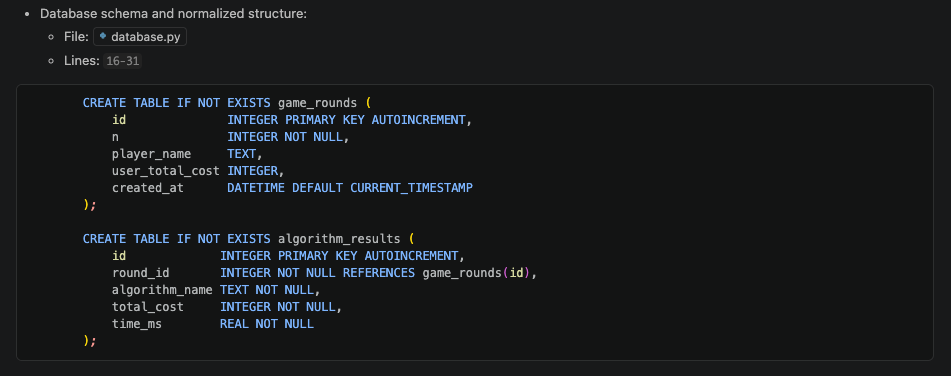
\includegraphics[width=0.95\linewidth]{database-schema-and-normalized-structure.png}
    \caption{The SQLite database schema layout.}
\end{figure}

\vspace{15cm} 

% ---------------------------------------------------------------------
\subsection{User Interface}
% ---------------------------------------------------------------------

\subsubsection{UI screenshot for inputs and answers}
The frontend was built using React and Vite. It has simple buttons for the users to choose how they want to play. You can either solve the problem manually by clicking cells in the matrix or let the computer do it for you.

\begin{figure}[H]
    \centering
    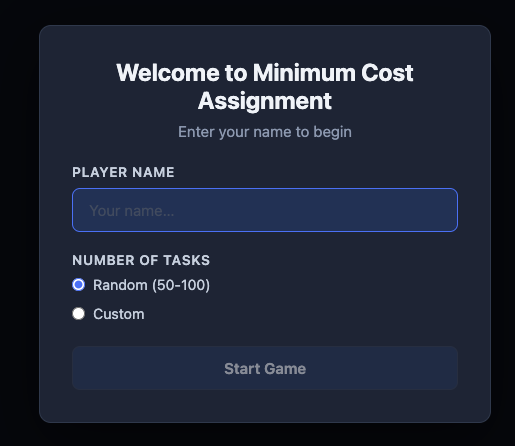
\includegraphics[width=0.75\linewidth]{username-input.png}
    \caption{This shows where the user types their name before starting.}
\end{figure}

\subsubsection{Validations and error handling}
We added several checks to make the app stable:
\begin{itemize}
    \item \textbf{Frontend (React)}: We made the UI so it prevents common mistakes. For example, you can't assign one worker to two different tasks by accident because the UI will automatically toggle the previous choice.
    \item \textbf{Backend (FastAPI)}: We use Pydantic models to check the data coming in. If the data is wrong or missing something, the backend sends an error instead of crashing. We also used try-except blocks in the database code to handle any SQL errors.
\end{itemize}


% ---------------------------------------------------------------------
\subsection{System Testing}
% ---------------------------------------------------------------------

\subsubsection{Unit Testing}
We used the pytest framework to test our code. We wrote several tests to make sure the algorithms work correctly. One important test was checking that the Hungarian algorithm always gives a cost that is less than or equal to the Greedy algorithm.

\begin{figure}[H]
    \centering
    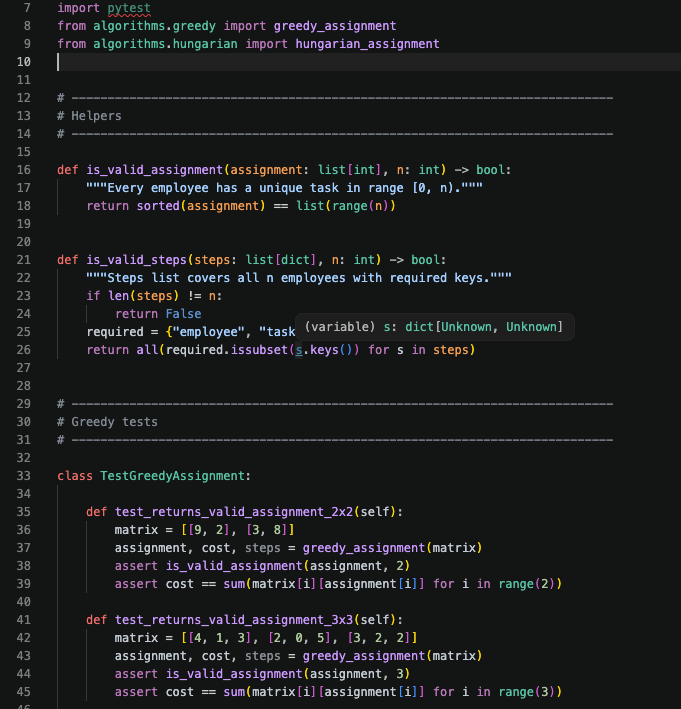
\includegraphics[width=0.95\linewidth]{unit-test-greedy.png}
    \caption{Testing our Greedy logic with pytest.}
\end{figure}

\begin{figure}[H]
    \centering
    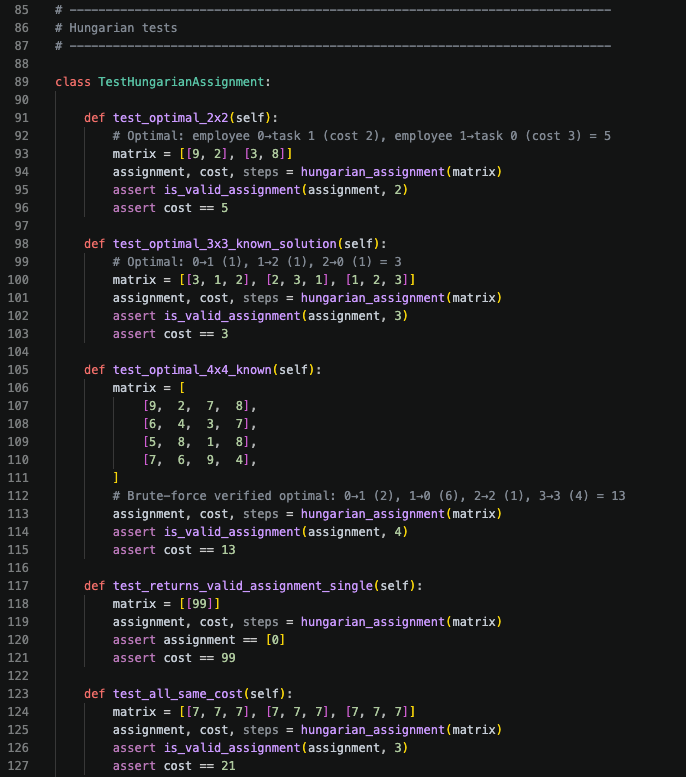
\includegraphics[width=0.95\linewidth]{unit-test-hungarian.png}
    \caption{Testing the Hungarian algorithm for correctness.}
\end{figure}

\newpage
% =====================================================================
\section{Appendix}
% =====================================================================

GitHub link - \url{https://github.com/adithyasean/game-project}

\vspace{1em}
All other deliverables are in this OneDrive link: 

\url{https://nibm-my.sharepoint.com/:f:/g/personal/cobsccomp242p-065_student_nibm_lk/IgC1z1sqJ0tgQ5aY-_paQP58ASlJvXpEXgEXOfWhQnmc9rQ?e=xGp5Ho}

\end{document}